%%%%%%%%%%%%%%%%%%%%%%%%%%%%%%%%%%%%%%%%%%%%%%%%%%%%%%%%%%%%%%%%%%%%%%%%
%                                                                      %
%     File: Thesis_Appendix_D.tex                                      %
%     Tex Master: Thesis.tex                                           %
%                                                                      %
%     Author: Israel Sother                                            %
%     Last modified: 27 May 2024                                       %
%                                                                      %
%%%%%%%%%%%%%%%%%%%%%%%%%%%%%%%%%%%%%%%%%%%%%%%%%%%%%%%%%%%%%%%%%%%%%%%%
\chapter{Inverter Design}
\label{chapter:appendix_inverter}

The new inverter design was intended to solve the current and voltage measurement issues that were present in the previous design, while also increasing the maximum current supported by the inverter. It was mainly designed using the same process as~\cite{Costa:MSc}. The design process started with the selection of the semiconductor devices based on an efficiency analysis, followed by the design of the gate drivers and the current and voltage measurement circuits. As this version of the inverter was intended to be used in the next prototypes, a special focus was given to reducing further the size of the inverter, while also making it more modular to allow for easier maintenance and replacement of components.

\section{Efficiency Equation Formulation}

To ease the process of choosing the semiconductor efficiency analysis approach was used. This was performed with the efficiency formulation for a three-phase inverter from~\cite{Costa:SiC_MOSFET_losses:2023}, as it represents well the system developed. In~\cite{Costa:SiC_MOSFET_losses:2023} the power loss is assumed to be majorly composed by the semiconductor losses, as the inverter does not have magnetic components. This assumption is based on~\cite{Song:SiC_MOSFET_losses:2019}, where it is stated that the power losses of SiC MOSFET chips in the power module account for more than 93.4\% of the total power losses of the power inverter.

The power losses of the MOSFET chips can be divided into conduction losses and switching losses defined as in~\cite{Costa:SiC_MOSFET_losses:2023}. The conduction losses are given by \Cref{eq:conduction_losses}.

\begin{equation}
	\frac{P_{ON}}{P_o} = \frac{R_{DS_{on}}}{R_0} (1+THD^2)
	\label{eq:conduction_losses}
\end{equation}

Where $P_{ON}$ is the conduction losses, $P_o$ is the output power, $R_{DS_{on}}$ is the on-state resistance of the MOSFET, $R_0$ is the load equivalent resistance and $THD$ is the total harmonic distortion of the output current.

The switching losses are presented in \Cref{eq:switching_losses}.

\begin{equation}
	\frac{P_{SW}}{P_o} = \left( \frac{\sqrt(3)}{2\pi m_p F_p}\frac{t_{on}+t_{off}}{T}+\frac{3 C_t Z_0}{m_p^2 F_p T} \right)(3-m_p)
	\label{eq:switching_losses}
\end{equation}

Where $P_{SW}$ is the switching losses,$Z_0$ is the load equivalent impedance defined as $Z_0 = \frac{R_0}{F_p}$ with $F_p$ being the load power factor, $t_{on}$ and $t_{off}$ are the turn-on and turn-off times of the MOSFET, $T$ is the switching period, $C_t$ is the total parasitic capacitance defined as $C_t = C_{oss} + C_d$ with $C_{oss}$ being the MOSFET output parasitic capacitance, and $C_d$ the external diode parasitic capacitance. The modulation index $m_p$ used in this formulation is different from the one used on the control scheme, and it is defined as $\sqrt{6} V_{ORMS}/V_{DC}$ where $V_{ORMS}$ is the line to neutral output RMS voltage.

The complete efficiency formulation is presented in \Cref{eq:efficiency}.

\begin{equation}
	\eta = \frac{1}{1 + \frac{P_{ON}}{P_o} + \frac{P_{SW}}{P_o}} = \frac{1}{1 + \frac{R_{DS_{on}}}{F_p Z_0} (1+THD^2) + \left( \frac{\sqrt{3}}{2\pi m_p F_p}\frac{t_{on}+t_{off}}{T}+\frac{3 C_t R_0}{m_p^2 F_p^2 T} \right)(3-m_p)}
	\label{eq:efficiency}
\end{equation}

\subsection{Motor and Controller parameters}
With the efficiency equation defined, the next step was to define the load parameters, in this case, the motor operation points. As the power factor of the motor changes with the motor speed and torque, a map of the power factor was used. This map is derived from manufacturer data and is presented in \Cref{fig:motor_power_factor}. As the manufacturer only provided the power factor for positive torque, the power factor for negative torque was assumed to be the same as the power factor for positive torque. While this is not accurate, it is a good approximation for the efficiency analysis.
\begin{figure}[H]
	\centering
	\begin{subfigmatrix}{2}
		\subfigure[Motor power factor.]{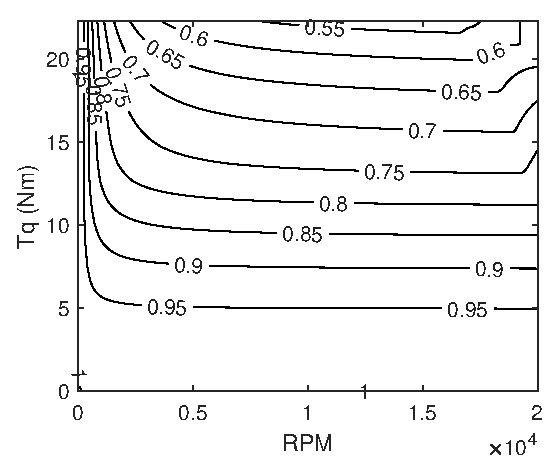
\includegraphics[width=0.45\linewidth]{Figures/motor_power_factor.eps}\label{fig:motor_power_factor}}
		\subfigure[Current THD.]{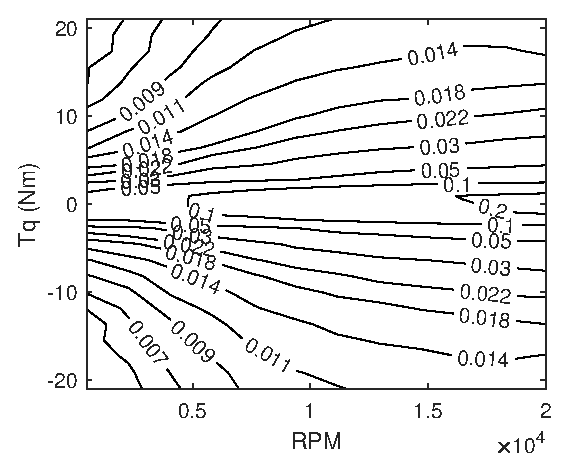
\includegraphics[width=0.45\linewidth]{Figures/THD_map.eps}\label{fig:THD_map}}
	\end{subfigmatrix}
	\caption{Motor power factor and current THD maps as a function of the motor speed and torque.}
	\label{fig:motor_power_factor_THD_map}
\end{figure}

The current \gls{thd} was calculated using the simulation environment presented in \Cref{section:simulation}. The motor was kept in a steady state for each of the operation points, and the current \gls{thd} was calculated. The results are presented in \Cref{fig:THD_map}.

\section{Operation Points}
As the load parameters are not constant a competition data-driven approach was taken to evaluate which module is better suited for the application. The logs from the 2023 competitions were used to create a 2-D histogram with the motor speed and torque usual operation points. \Cref{fig:motor_operation_points} presents the histogram of the operation points for each motor in the 2023 \gls{fsg} Endurance Event as an example.

\begin{figure}[H]
	\centering
	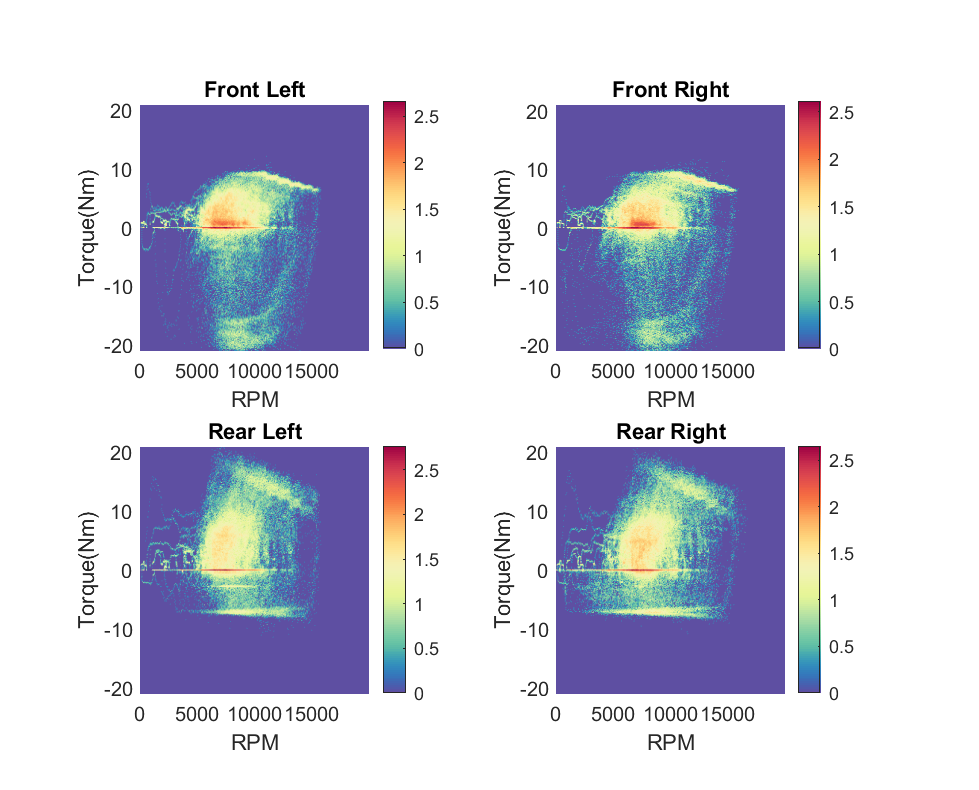
\includegraphics[trim=1cm 0.3cm 1.6cm 1cm, clip, width=0.8\textwidth]{Figures/Endurance_FSG_4wd.eps}
	\caption{Motor operation points for the 2023 Germany Endurance Event. The color represents the number of points in each bin on a logarithmic scale.}
	\label{fig:motor_operation_points}
\end{figure}

To generalize the design, each of the motor's operation points was combined, resulting in a single histogram with the operation points of all the motors. An example of the combined histogram is presented in \Cref{fig:motor_operation_points_combined}.

\begin{figure}[H]
	\centering
	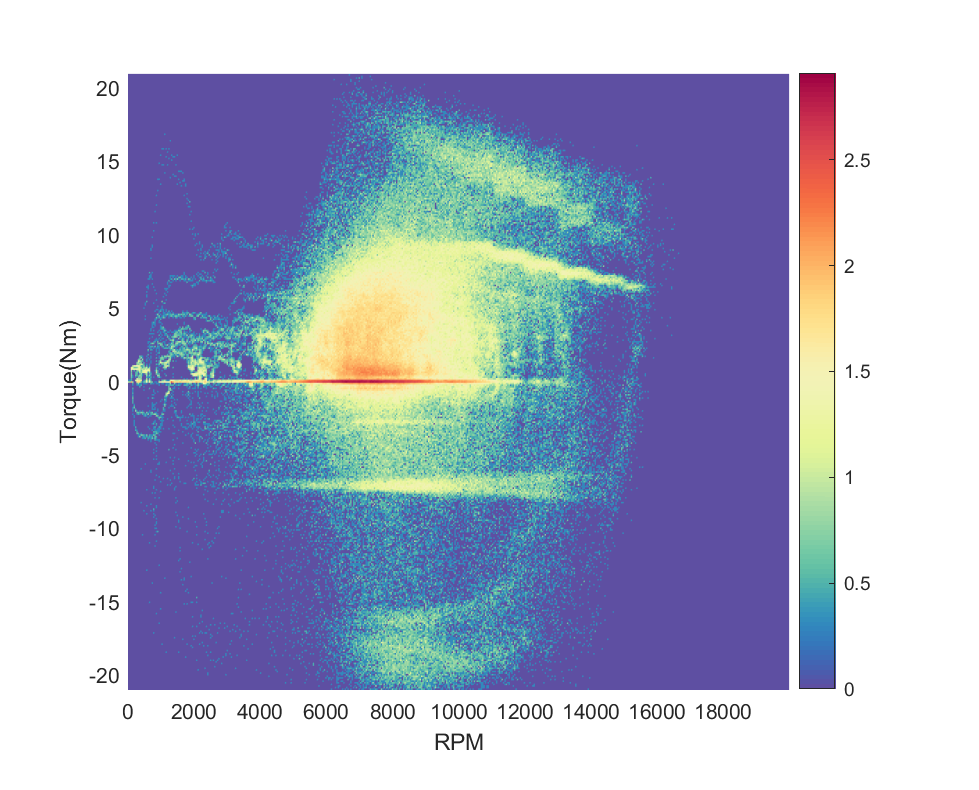
\includegraphics[width=0.8\textwidth]{Figures/Endurance_FSG_combined.eps}
	\caption{Combined motor operation points for the 2023 Germany Endurance Event. The color represents the number of points in each bin on a logarithmic scale.}
	\label{fig:motor_operation_points_combined}
\end{figure}

With the operation points defined, the efficiency of the inverter was averaged using the operation points histogram as weights. This allowed a direct comparison of the average efficiency of each semiconductor in a representative competition environment. The results for the chosen module are presented in \Cref{fig:efficiency_inverter}.

\section{Diode Selection}
The antiparallel diode is used with two main functions, the first is to protect the MOSFETs from the reverse voltage generated by the motor inductance in case a fault occurs and the control shuts down the inverter while the motor is still spinning. Although in this case, the MOSFET body diode would allow the current to flow, it usually has a smaller forward current rating and a high forward voltage drop, thus in a failure mode it would heat the module and possibly damage it. The second reason is related to efficiency, as it allows the current that would flow through the MOSFET body diode to flow through the external diode, which has a smaller forward voltage drop, thus reducing the conduction losses in the dead time period.
To select the proper diode to parallel with the MOSFETs, the principal factors are the diode must support at least double the DC Link voltage in reverse voltage, and the peak current of the diode must be at least the peak current of the motor. The continuous current rating is not a concern here because in normal operation as soon as the MOSFET is turned on the diode will not conduct any current, as the MOSFET resistance produces a voltage drop smaller than the forward voltage of the diode. Ideally, the diode would be dimensioned to endure the peak current for the longest fault mode, but timing constraints prevented this study from being made, so it was dimensioned by the normal operation conditions of the motor datasheet~\cite{amk:DD5-14-10-POW}. The diode should also have a small parasitic capacitance to reduce the increase in the switching losses, and a low forward voltage drop to reduce the conduction losses in the dead time period.

\Cref{tab:diode_list} presents the list of possible diodes for the new inverter design compared with the one used on the current design.
\begin{table}[H]
	\centering
	\caption{List of possible diodes for the new inverter design compared to the solution used on the current design.}
	\label{tab:diode_list}
	\resizebox{\textwidth}{!}{%
	\begin{tabular}{ccccccccc}
		\toprule
		\textbf{Manufacturer} & \textbf{Model}    & \textbf{$\mathbf{V_{RRM}(V)}$} & \textbf{$\mathbf{V_f(V)}$} & \textbf{$\mathbf{I_f(A)}$} & \textbf{$\mathbf{I_{fsm}(A)}$} & \textbf{$\mathbf{C(pF)}$} & \textbf{$\mathbf{T_{MAX}(\degree C)}$} & \textbf{Price (\texteuro)} \\ \midrule
		ST			& STBR3012-Y        & 1200	& 0.95	& 30	& 300	& 15	& 175	& 2.62  	\\ 
		Littelfuse	& LSIC2SD120D15     & 1200	& 1.5	& 44	& 120	& 76	& 175	& 10.5  	\\ 
		Microchip	& MSC050SDA120B     & 1200	& 1.5	& 109	& 290	& 214	& 175	& 16.6  	\\ 
		GeneSiC		& GD60MPS17H        & 1700	& 1.5	& 122	& 600	& 252	& 175	& 42.85  	\\
		Vishay		& VS-E5TH3012S2L-M3 & 1200	& 1.9	& 30	& 240	& 17	& 175	& 2.76  	\\ \midrule
		Cree		& C4D10120E         & 1200	& 1.5	& 33	& 75	& 41.5	& 175	& 11.53  	\\ \bottomrule
	\end{tabular}%
}
\end{table}

Due to its reduced cost and good performance, the ST STBR3012-Y was chosen for the new inverter design. While this is not a SiC diode, it still fulfills the requirements for the application and presents the best performance on paper.

\section{MOSFET Module Selection}


To increase the inverter density and improve the thermal performance the semiconductors were limited to half-bridge modules, as they allow for a more compact design and easy integration, while also reducing the number of components needed. The use of the half-bridge configuration was also motivated by the modularity provided, as this simplifies the design to one inverter leg that can be replicated to compose the complete inverter. This modularity also allows for easier maintenance and replacement of components, at the cost of the reduced number of available semiconductors in the market.

As the battery voltage currently used is 600V, the semiconductors needed to have a voltage rating of at least 1200V. The maximum motor current is approximately $150A$, with a nominal current of $45A_{RMS}$, setting the minimum drain current rating of the MOSFETs to $45A$. The other parameters can be reasonably selected to maximize the efficiency of the inverter. Based on these initial requirements a list of possible MOSFETs was created and shown in \Cref{tab:mosfet_list}. Note that the 1700V semiconductors are significantly more expensive than the 1200V semiconductors, thus they are not considered for the final design.  The Microchip modules include Schottky diodes, while the other modules do not include the diodes, thus in the efficiency calculations the capacitance of the chosen diode was summed to the other modules to allow for a fair comparison.

% Please add the following required packages to your document preamble:
% \usepackage{graphicx}
\begin{table}[]
	\centering
	\caption{List of possible MOSFET modules for the new inverter design compared to the discrete solution used on the current design.}
	\label{tab:mosfet_list}
	\resizebox{\textwidth}{!}{%
		\begin{tabular}{ccccccccccccc}
			\toprule
			\textbf{Manufacturer} & \textbf{Model}             & \textbf{$\mathbf{V_{DSS} (V)}$} & \textbf{$\mathbf{R_{DS_{on}}(m\Omega)}$} & \textbf{$\mathbf{I_d(A)}$} & \textbf{$\mathbf{T_{max} \degree C}$} & \textbf{$\mathbf{C_{OSS}(pF)}$} & \textbf{$\mathbf{t_{on}(ns)}$} & \textbf{$\mathbf{t_{off}(ns)}$} & \textbf{Price (\texteuro)} \\ \midrule
			Infineon      & FF4MR12W2M1HP\_B11         & 1200    & 4       & 200     & 175     & 840      & 44      & 16      & 260.85   \\ 
			Infineon      & FF6MR12W2M1H\_B11          & 1200    & 5.4     & 150     & 175     & 630      & 39      & 15      & 194.88   \\ 
			Infineon      & FF08MR12W1MA1\_B11A        & 1200    & 7.33    & 150     & 150     & 700      & 35      & 38      & 268.99   \\ 
			Infineon      & FF8MR12W1M1H\_B11          & 1200    & 8.1     & 100     & 175     & 420      & 70      & 20      & 165.21   \\ 
			Infineon      & FF11MR12W2M1HP\_B11        & 1200    & 10.8    & 100     & 150     & 315      & 41.1    & 21.2    & 125.12   \\ 
			Microchip     & MSCSM170AM11CT3AG          & 1700    & 8.8     & 240     & 175     & 600      & 17      & 19      & 499.29   \\ 
			Microchip     & MSCSM170AM15CT3AG          & 1700    & 11.7    & 181     & 175     & 450      & 17      & 19      & 425.52   \\ 
			Microchip     & MSCSM120AM11CT3AG          & 1200    & 10.4    & 254     & 175     & 810      & 30      & 25      & 360.10   \\ 
			Microchip     & MSCSM120AM16CT1AG          & 1200    & 16      & 173     & 175     & 540      & 30      & 25      & 206.89   \\ 
			Semikron      & SK150MB120CR03TE2          & 1200    & 8       & 188     & 175     & 520      & 17      & 29      &          \\ 
			Vincotech     & 10-EZ122PA016ME-LJ67F68T   & 1200    & 17      & 83      & 175     & 258      & 6.72    & 21.48   &          \\ 
			Vincotech     & 10-EY122PA008ME01-LU38F06T & 1200    & 9.11    & 184     & 175     & 516      & 40      & 16.92   &          \\ \midrule
			Wolfspeed     & C2M0040120D                & 1200    & 44      & 55      & 150     & 171      & 61      & 13      & 45.94    \\ \bottomrule
		\end{tabular}%
	}
\end{table}

For each semiconductor in the list, an efficiency map was created using the efficiency formulation presented in \Cref{eq:efficiency}, and the operation points histogram presented in \Cref{fig:motor_operation_points_combined} was used to compute the average efficiency throughout the last \gls{fsg} Endurance event. The average results are presented in \Cref{tab:efficiency_comparison}.

\begin{table}[]
	\centering
	\caption{Efficiency comparison of the possible MOSFETs modules for the new inverter design.}
	\label{tab:efficiency_comparison}
	\resizebox{\textwidth}{!}{%
	\begin{tabular}{cccccc}
		\toprule		
		\textbf{Manufacturer} & \textbf{Model}             & \begin{tabular}[c]{@{}c@{}}\textbf{Conduction} \\ \textbf{Loss (W)}\end{tabular} &  \begin{tabular}[c]{@{}c@{}}\textbf{Switching} \\ \textbf{Loss (W)}\end{tabular}& \textbf{Efficiency (\%)} & \textbf{Price (\texteuro)} \\ \midrule
		Microchip             & MSCSM120AM16CT1AG          & 70.80         & 15.53  & 98.76      & 206.89         \\
		Vincotech             & 10-EZ122PA016ME-LJ67F68T   & 75.22         & 7.94   & 98.80      &                \\
		Infineon              & FF11MR12W2M1HP\_B11        & 47.78         & 15.66  & 99.08      & 125.12         \\
		Microchip             & MSCSM120AM11CT3AG          & 46.02         & 17.38  & 99.08      & 360.10         \\
		Microchip             & MSCSM170AM15CT3AG          & 51.77         & 10.83  & 99.09      & 425.52         \\
		Infineon              & FF8MR12W1M1H\_B11          & 35.84         & 22.34  & 99.16      & 165.21         \\
		Vincotech             & 10-EY122PA008ME01-LU38F06T & 40.31         & 15.88  & 99.19      &                \\
		Infineon              & FF08MR12W1MA1\_B11A        & 32.43         & 20.60  & 99.23      & 268.99         \\
		Microchip             & MSCSM170AM11CT3AG          & 38.94         & 11.85  & 99.26      & 499.29         \\
		Semikron              & SK150MB120CR03TE2          & 35.40         & 13.56  & 99.29      &                \\
		Infineon              & FF6MR12W2M1H\_B11          & 23.89         & 16.03  & 99.42      & 194.88         \\
		Infineon              & FF4MR12W2M1HP\_B11         & 17.70         & 18.76  & 99.47      & 260.85         \\ \midrule
		Wolfspeed             & C2M0040120D                & 194.69        & 17.19  & 97.00      & 45             \\ \bottomrule
	\end{tabular}
	}
\end{table}

Although it does not have the highest efficiency, the Infineon FF8MR12W1M1H\_B11~\cite{Infineon:Module_Datasheet:2023} was chosen as it has one of the smallest footprints, while having good efficiency and a reasonable price.  It also brings significant performance gains when compared to the discrete option used on the current inverter design that averaged at $97\%$ efficiency, and even more when compared with the inverter currently used on the vehicle, which averages at only $86\%$. One interesting factor to note here is the dominance of the conduction losses over the switching losses, indicating an increase in switching frequency could be beneficial to the efficiency of the inverter as it would reduce the current \gls{thd} and thus the conduction losses. The resulting inverter efficiency is presented in \Cref{fig:efficiency}.

% \begin{figure}[H]
% 	\centering
% 	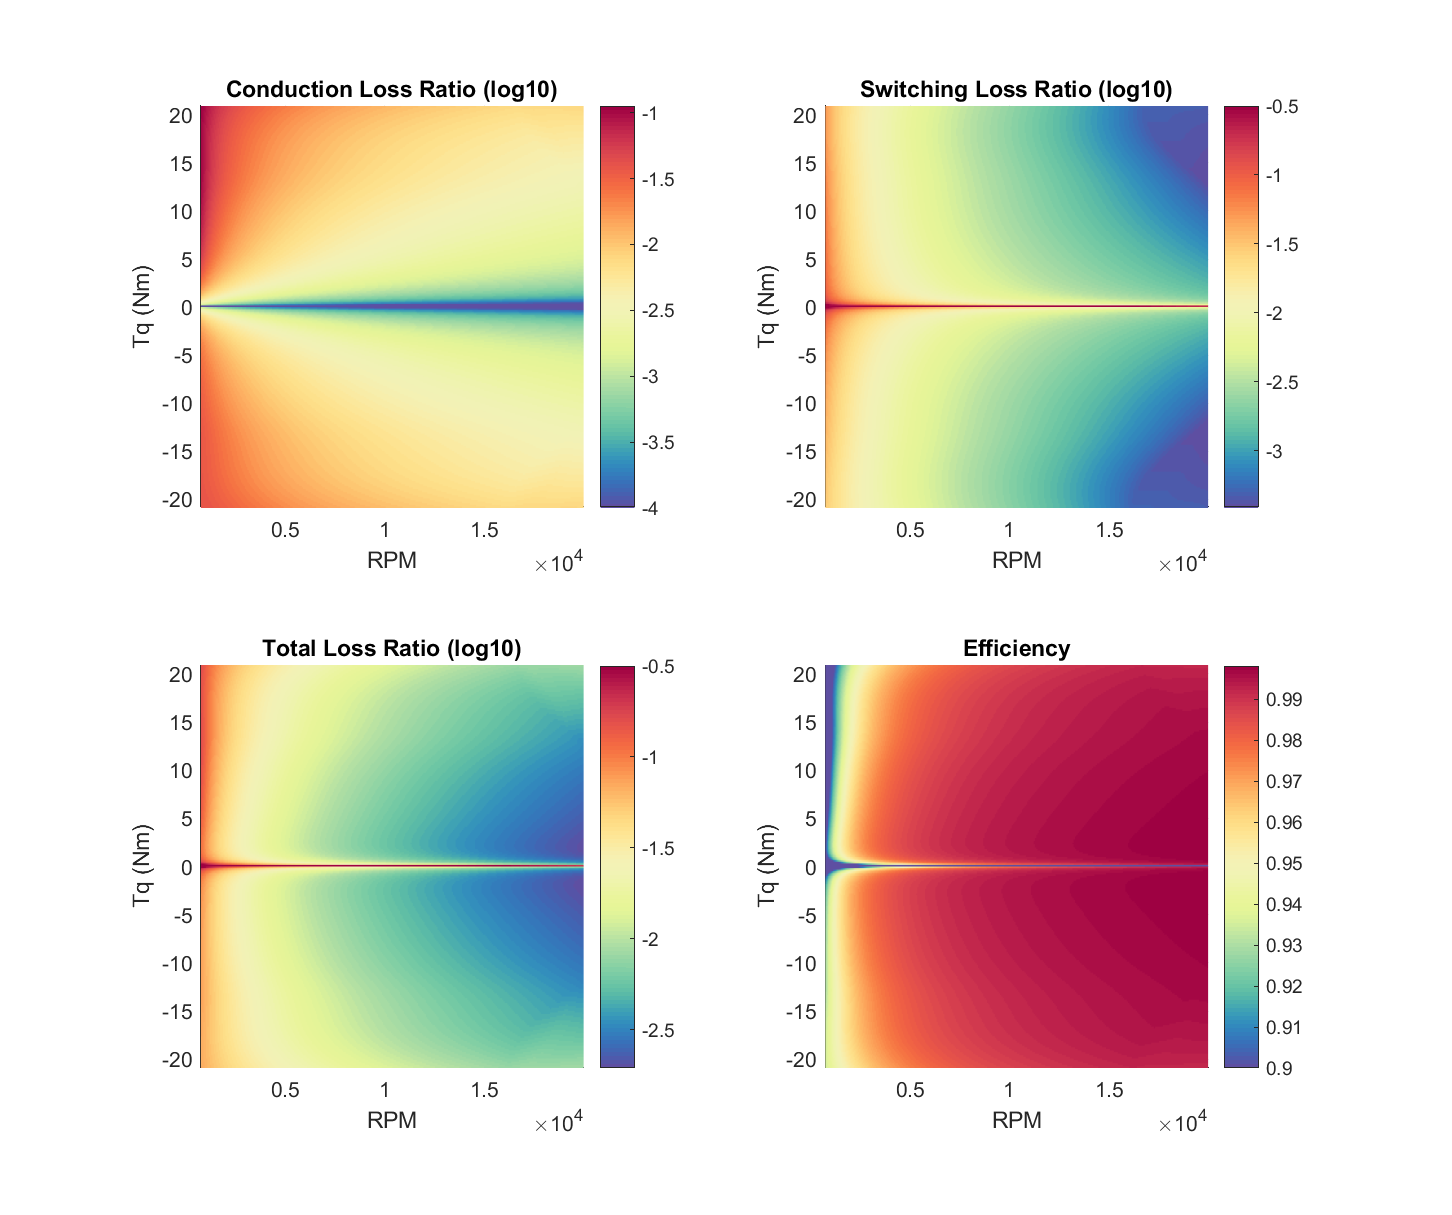
\includegraphics[width=1\textwidth]{Figures/Infineon-FF8MR12W1M1H_B11_eff.eps}
% 	\caption{Ratio of Conduction and Switching losses against output power, and overall inverter efficiency using the Infineon FF8MR12W1M1H\_B11 module.}
% 	\label{fig:efficiency_inverter}
% \end{figure}

\pgfplotsset{
	contour/label node code/.code={%
		\node at (axis direction cs: 3200pt,0pt){$ $\pgfmathprintnumber{#1} $\%$};%
	}%
}

\begin{figure}[H]
	\centering
	\begin{subfigmatrix}{2}
		\subfigure[Conduction Loss Ratio.]{
			\begin{tikzpicture}
				\begin{axis}[
					height=7cm,
					width=0.45\linewidth,
					view={0}{90},
					mesh/ordering=x varies,
					mesh/cols=49,
					mesh/rows=60,
					xtick={4000,8000,12000,16000,20000},
					ymin=-21,
					ymax=21,
					xmin=700,
					xmax=20000,
					point meta min=-5, 
					point meta max=5,
					xlabel={RPM},
					ylabel={Torque (Nm)},
					shader=interp]
					\addplot3[samples=100, contour gnuplot={levels = {5,2,1,0.6,0.3,0.05},draw color=black,contour label style={every node/.append style={text=black}}},contour/draw color={black},contour/label distance=110pt] table[skip first n=2,x=x, y=y, z=z] {Figures/subplot_1.dat};
				\end{axis}
			\end{tikzpicture}
			\label{fig:cond_loss_ratio}
		}
		\subfigure[Switching Loss Ratio.]{
			\pgfplotsset{
				contour/label node code/.code={%
					\node at (axis direction cs: 0pt,0pt){$ $\pgfmathprintnumber{#1} $\%$};%
				}%
			}
			\begin{tikzpicture}
				\begin{axis}[
					height=7cm,
					width=0.45\linewidth,
					view={0}{90},
					mesh/ordering=x varies,
					mesh/cols=43,
					mesh/rows=60,
					xtick={4000,8000,12000,16000,20000},
					ymin=-21,
					ymax=21,
					xmin=700,
					xmax=20000,
					point meta min=-5, 
					point meta max=5,
					xlabel={RPM},
					ylabel={Torque (Nm)},
					shader=interp]
					\addplot3[samples=100, contour gnuplot={levels = {1.5,0.6,0.3,0.15,0.05},draw color=black,contour label style={every node/.append style={text=black}}},contour/draw color={black},contour/label distance=120pt] table[skip first n=2,x=x, y=y, z=z] {Figures/subplot_2.dat};
				\end{axis}
			\end{tikzpicture}
			\label{fig:sw_loss_ratio}
		}
	\end{subfigmatrix}
	\begin{subfigmatrix}{2}
		\subfigure[Total Loss Ratio.]{
			\begin{tikzpicture}
				\begin{axis}[
					height=7cm,
					width=0.45\linewidth,
					view={0}{90},
					mesh/ordering=x varies,
					mesh/cols=45,
					mesh/rows=60,
					xtick={4000,8000,12000,16000,20000},
					ymin=-21,
					ymax=21,
					xmin=700,
					xmax=20000,
					point meta min=-5, 
					point meta max=5,
					xlabel={RPM},
					ylabel={Torque (Nm)},
					shader=interp]
					\addplot3[samples=100, contour gnuplot={levels = {5,3,1.5,1,0.5,0.25,0.05},draw color=black,contour label style={every node/.append style={text=black}}},contour/draw color={black},contour/label distance=140pt] table[skip first n=2,x=x, y=y, z=z] {Figures/subplot_3.dat};
				\end{axis}
			\end{tikzpicture}
			\label{fig:total_loss_ratio}
		}
		\subfigure[Efficiency.]{
			\begin{tikzpicture}
				\begin{axis}[
					height=7cm,
					width=0.45\linewidth,
					view={0}{90},
					mesh/ordering=x varies,
					mesh/cols=45,
					mesh/rows=60,
					xtick={4000,8000,12000,16000,20000},
					ymin=-21,
					ymax=21,
					xmin=700,
					xmax=20000,
					point meta min=-5, 
					point meta max=5,
					xlabel={RPM},
					ylabel={Torque (Nm)},
					shader=interp]
					\addplot3[samples=100, contour gnuplot={levels = {95,97.5,98.5,99,99.25,99.5,99.7},draw color=black,contour label style={every node/.append style={text=black}}},contour/draw color={black},contour/label distance=200pt] table[skip first n=2,x=x, y=y, z=z] {Figures/subplot_4.dat};
				\end{axis}
			\end{tikzpicture}
			\label{fig:efficiency}
		}
	\end{subfigmatrix}
	\caption{Render of the PCBs used in the new inverter design.}
	\label{fig:pcb_render}
\end{figure}

\pgfplotsset{
	contour/label node code/.code={%
		\node at (axis direction cs: -50pt,0pt){$ $\pgfmathprintnumber{#1} $\%$};%
	}%
}


\section{Gate Driver Design}

The selection of the gate driver was based on models proposed by the manufacturer, with the key aspects being a high source/sink current capability, galvanic isolation, and a fast desaturation function. The selected device was the Infineon EiceDRIVER™ 1ED332xMC12N~\cite{Infineon:GateDriver_Datasheet:2023}, but as the design was defined to have the main gate driver on a mezzanine board, a secondary gate driver was needed to be placed next to the module on the power module and reduce the parasitic inductance of the gate driver connections. The secondary gate driver does not need such strict requirements, only requiring a high source/sink current capability, as the desaturation function and isolation are already present on the main gate driver. The selected secondary gate driver was the Texas Instruments UCC27614~\cite{TexasInstruments:GateDriver_Datasheet:2022}, as it can provide 10A of source/sink current, can whitsdant the -5 to 18V voltage range of the primary gate driver, while having a small 8-Pin SON DSG footprint.

The gate resistance was chosen using the recommended values from the datasheet of the MOSFETs module, set in $8.2\Omega$ for charging and $2.7\Omega$ for discharging the gate. One drawback of using this cascaded gate driver approach is the increased impedance seen by the primary gate driver, as the secondary gate driver has an input impedance of $120k\Omega$, which makes this signal extremely sensitive to noise. To mitigate this issue, a strong pull-down resistor was added near the secondary gate driver input to reduce the impedance seen by the primary gate driver. A $5.6k\Omega$ resistor was chosen, as this is the smallest resistance value that does not exceed the maximum power dissipation of a 0603 resistor. A low-pass filter was also added to the gate driver input after the pull-down, with a cutoff frequency of $4.8229MHz$ to increase noise immunity. \Cref{eq:gate_energy_vs_capacitor} was used to calculate the decoupling capacitor value that would allow a voltage ripple smaller than $1\%$. In this equation $Q_g$ is the gate charge of the MOSFETs, $V_s$ is the supply voltage swing of the gate driver, $C_{decoupling}$ is the decoupling capacitance, $V_{initial}$ is the initial voltage of the capacitor, and $V_{final}$ is the final voltage of the capacitor. The resultant value was $5\mu F$, but a smaller $100nF$ was added in parallel to account for high-frequency oscillations.

\begin {equation}
	E = Q_g V_s = \frac{1}{2} C_{decoupling} (V_{initial}^2 - V_{final}^2)
	\label{eq:gate_energy_vs_capacitor}
\end{equation}

The short circuit protection of the MOSFETs was made using the desaturation function of the primary module, the used circuit is shown on \Cref{fig:desat_circuit}. The desaturation function is a protection mechanism that detects the voltage drop on the MOSFETs when they are on, and if this voltage drop is higher than a certain threshold, the gate driver turns off the MOSFETs. This is a very important protection mechanism, as it can prevent the MOSFETs from being destroyed in case of a short circuit.

\begin{figure}[H]
	\centering
	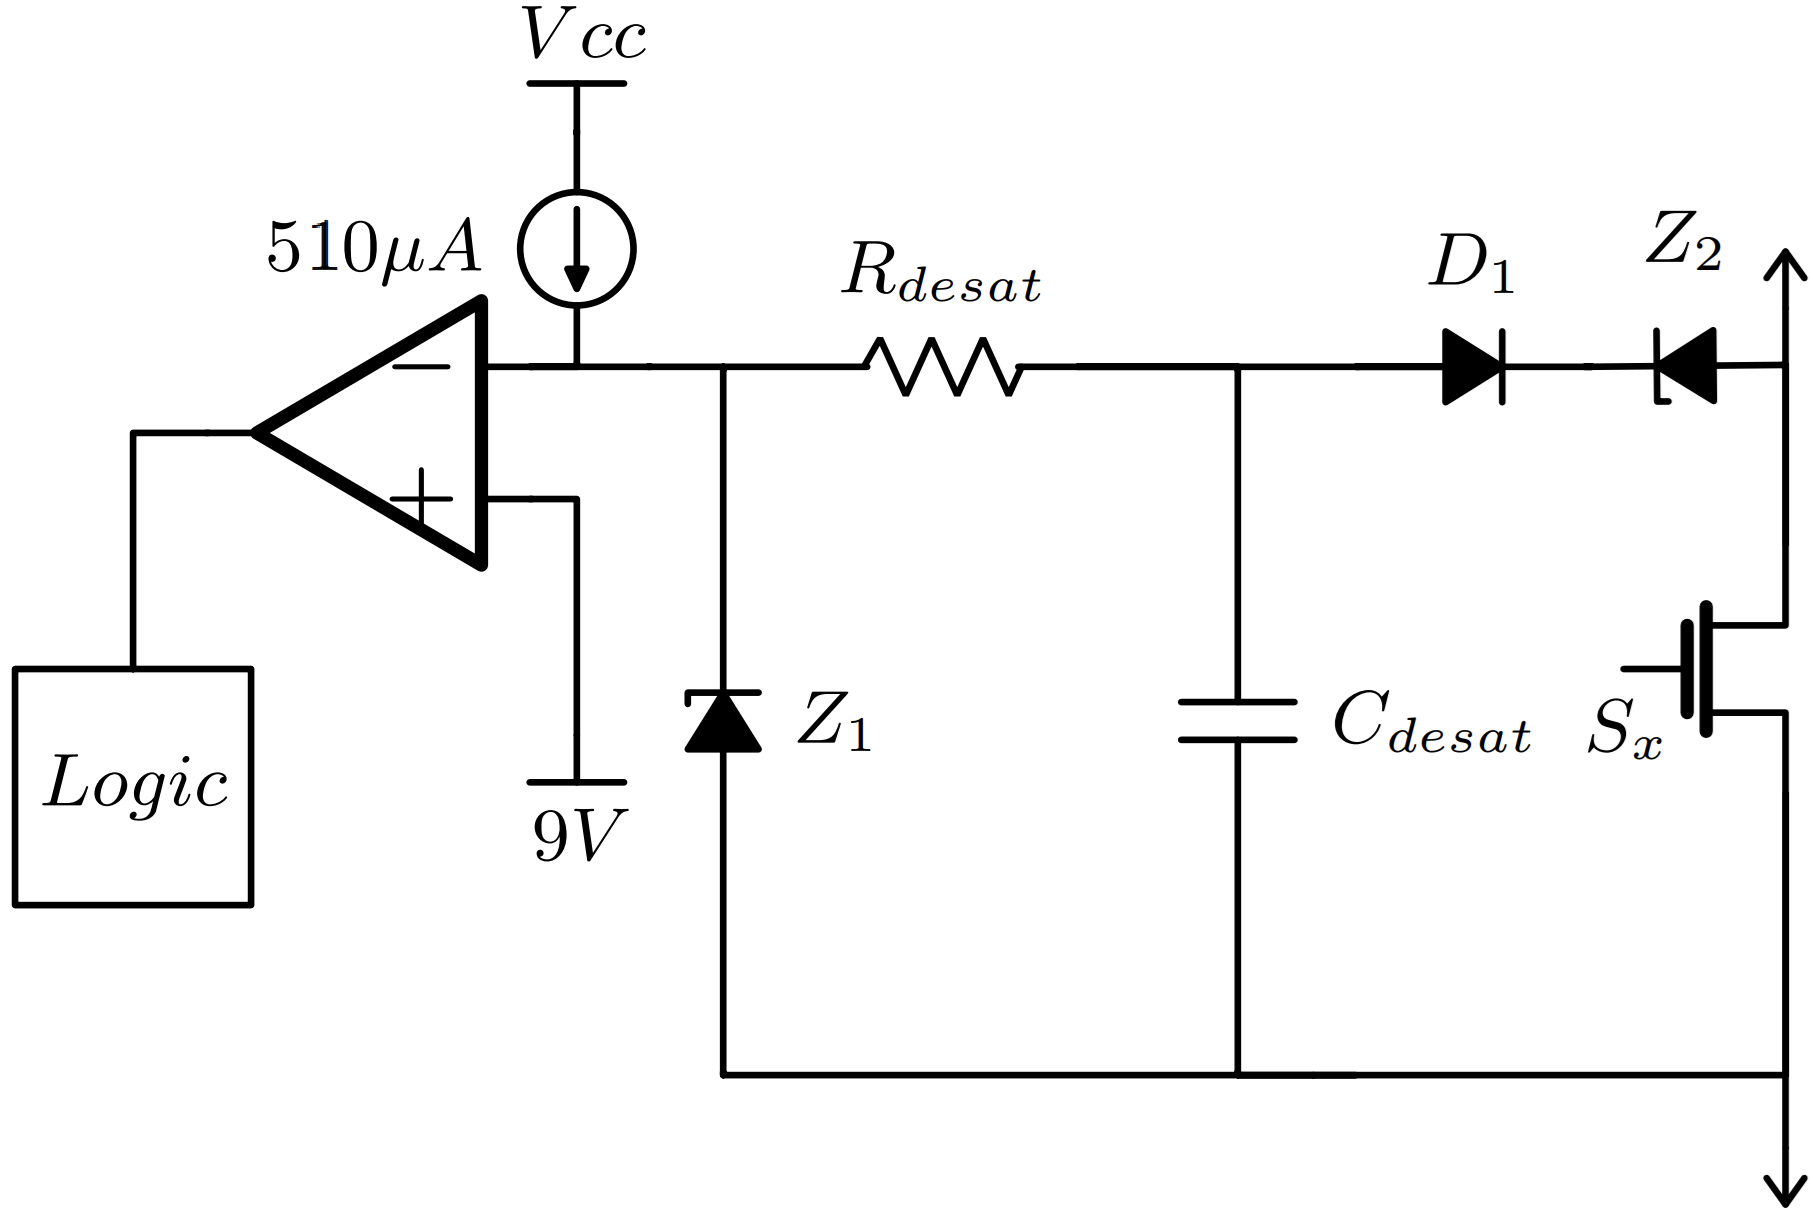
\includegraphics[width=0.5\textwidth]{Figures/desat_circuit.png}
	\caption{Desaturation protection circuit (adapted from~\cite{Costa:MSc}).}
	\label{fig:desat_circuit}
\end{figure}

The threshold voltage of the desaturation on the primary gate driver is $9V$, so the Zener diode $Z_2$ was used to produce a higher voltage drop and trigger the desaturation function with a lower current. The MOSFET datasheet details the $V_{DS}$ with different drain currents and gate voltages, based on that it was verified that at room temperature the MOSFET has a $V_{DS}$ of $1V$ with a $120A$ drain current. As the module heats up this voltage drop is reached with lower currents, thus it has a negative feedback that ensures the current will not exceed $120A$. As the diode $D_1$ has a forward voltage drop of $1V$ at room temperature, $Z_2$ should have a Zener voltage of $7V$, summing up to the $9V$ reference voltage of the gate driver. This is a very conservative current limit to start the design tests, but as the team's confidence in the design is increased, the Zenner voltage can be decreased to allow higher currents. 

The desaturation function has a blanking time to account for short bursts of current in normal operation, this blanking time is defined by the resistor $R_{desat}$ and the capacitor $C_{desat}$. They were dimensioned by \Cref{eq:desat_time} to have a blanking time of $3.8\mu s$. 

\begin {equation}
	t_{desat} = \frac{V_{ref} C_{desat}}{I_{desat}}
	\label{eq:desat_time}
\end{equation}
\section{Current and Voltage Measurement}

The design of the current and voltage sense was focused on increasing its noise immunity, as the previous design had issues with the current measurement. The current sensor was chosen to be the LEM LA 100-P~\cite{LEM:Current_sensor_datahseet:2018}, as it's a compact solution that can measure up to $150A$ with low drift and linearity error while having the bandwidth necessary for the fast controller frequency. Another advantage of this sensor is that it does not use integrated conductors, it only needs to wrap the primary conductor with the sensor, and as such, the current sense board does not need to be designed for high currents. This sensor outputs a current in the secondary circuit proportional to the primary circuit current, so a measurement resistance was set to $33\Omega$ as recommended by the manufacturer.

The output voltage is amplified and converted to a differential signal by a low drift operational amplifier with passive and active low pass filters, both with a cutoff frequency of $72.3kHz$. This signal conditioning was placed as close as possible to the sensor output to reduce \gls{emi} in the readings. Next to the signal conditioning circuitry, a 14-bit SAR ADC was placed to read the sensor output. This multichannel ADC is also used to read the voltage and temperature sensors. Its output is sent to the main controller through an RS-485 communication interface.

The voltage sense is done using a voltage divider followed by an isolated amplifier that also is coupled with an active lowpass filter. The voltage divider has a configurable input that allows selecting the module to measure DC Link voltage or motor phase voltage. This ability to measure the motor voltage was implemented to enable future automatic characterization routines.

\section{PCB Design}

The PCB was designed with creepage distances according to IPC2221A~\cite{IPC-2221:1998} to withstand the maximum battery voltage. One of the main goals in the PCB design was to keep the solution compact, and to achieve that a mezzanine approach was selected. This approach allowed the leg module to be designed within the size of the MOSFET module, reducing the size of the inverter and allowing for great liberty with how the modules are arranged by the team inside the inverter container. 

The design is comprised of three main boards: Half-Bridge, Driver, and Current sense boards. The Half-Bridge board is the only board carrying high currents in the inverter, it contains the MOSFETs, DC Link capacitors, and the secondary gate drivers. It uses a 8-layer stack-up with copper thicknesses of $70\mu m$ on external layers and $35\mu m$ on internal layers. The use of 8 layers allowed to increase the current carrying capability of the board, being able to stand a current of $90A$ continuously. The Driver board contains the primary gate driver, the isolated DC/DCs to supply the gate drivers, and the isolation components for the voltage and temperature measurement. It also handles the connection with the other boards and the main controller. The Current sense board contains the current sensor coupled with the signal conditioning circuitry. It also includes the ADC to read all the module sensors and the communication interface with the main controller. The communication is done using RS-485, as it is a robust communication protocol that can be used in noisy environments. A render of each board and the final leg module is presented in \Cref{fig:pcb_render,fig:inverter_leg_render}.

\begin{figure}[H]
	\centering
	\begin{subfigmatrix}{2}
		\subfigure[Half-Bridge board.]{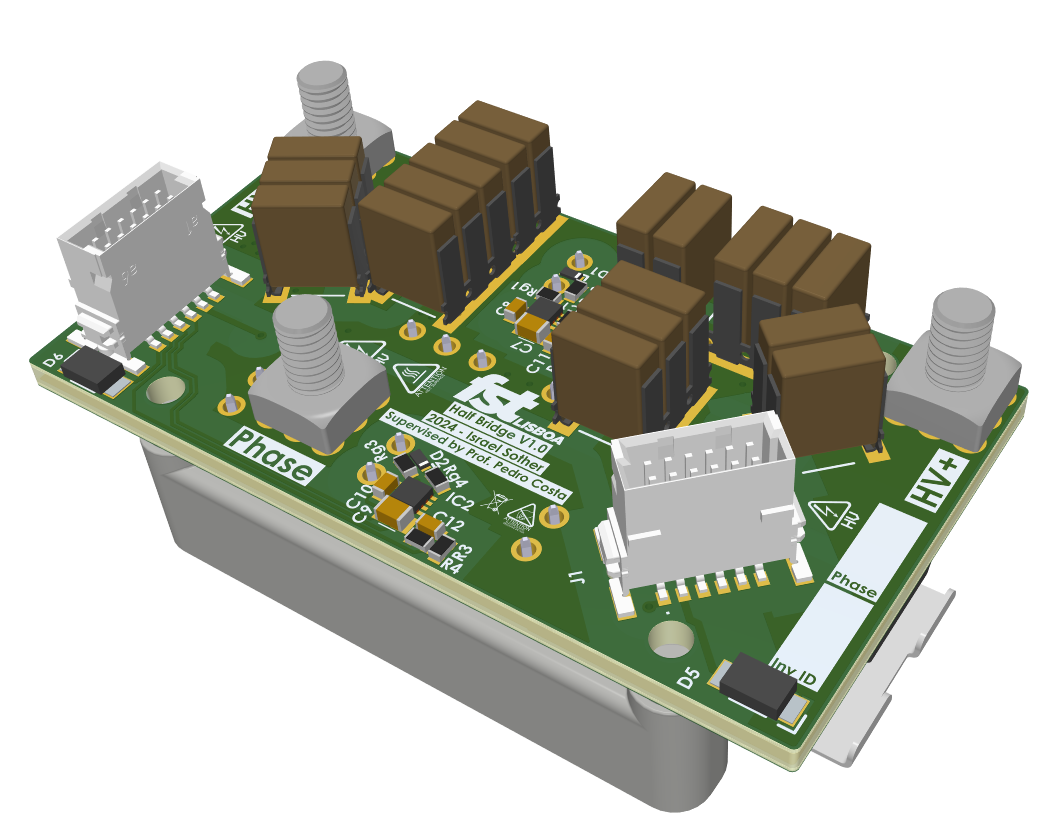
\includegraphics[width=0.48\linewidth]{Figures/Half Bridge.png}\label{fig:half_bridge_board}}
		\subfigure[Driver board.]{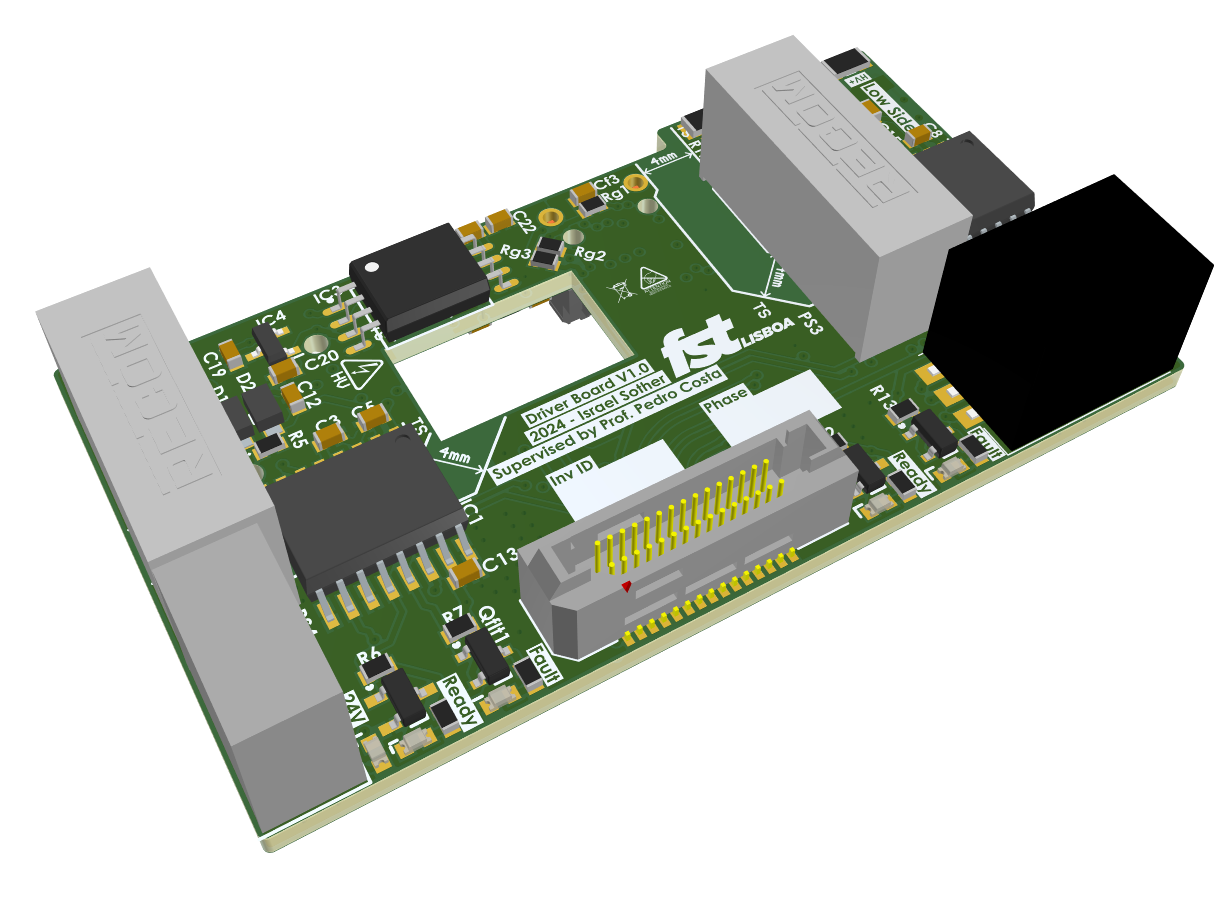
\includegraphics[width=0.48\linewidth]{Figures/Driver_Board.png}\label{fig:driver_board}}
	\end{subfigmatrix}
	\begin{subfigmatrix}{1}
		\subfigure[Current sense board.]{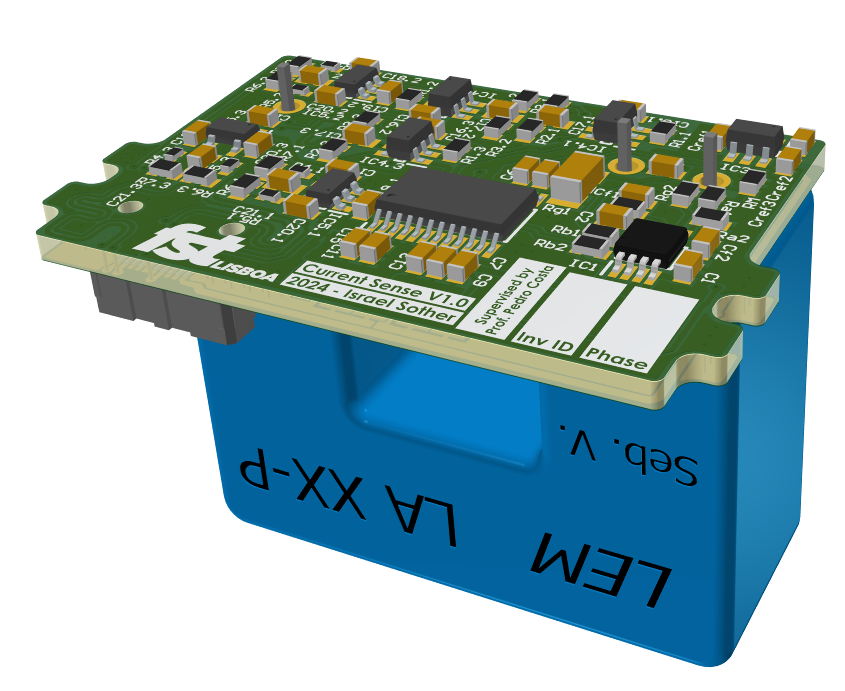
\includegraphics[width=0.5\linewidth]{Figures/Curr_Sensor.png}\label{fig:current_sense_board}}
	\end{subfigmatrix}
	\caption{Render of the PCBs used in the new inverter design.}
	\label{fig:pcb_render}
\end{figure}

\begin{figure}[H]
	\centering
	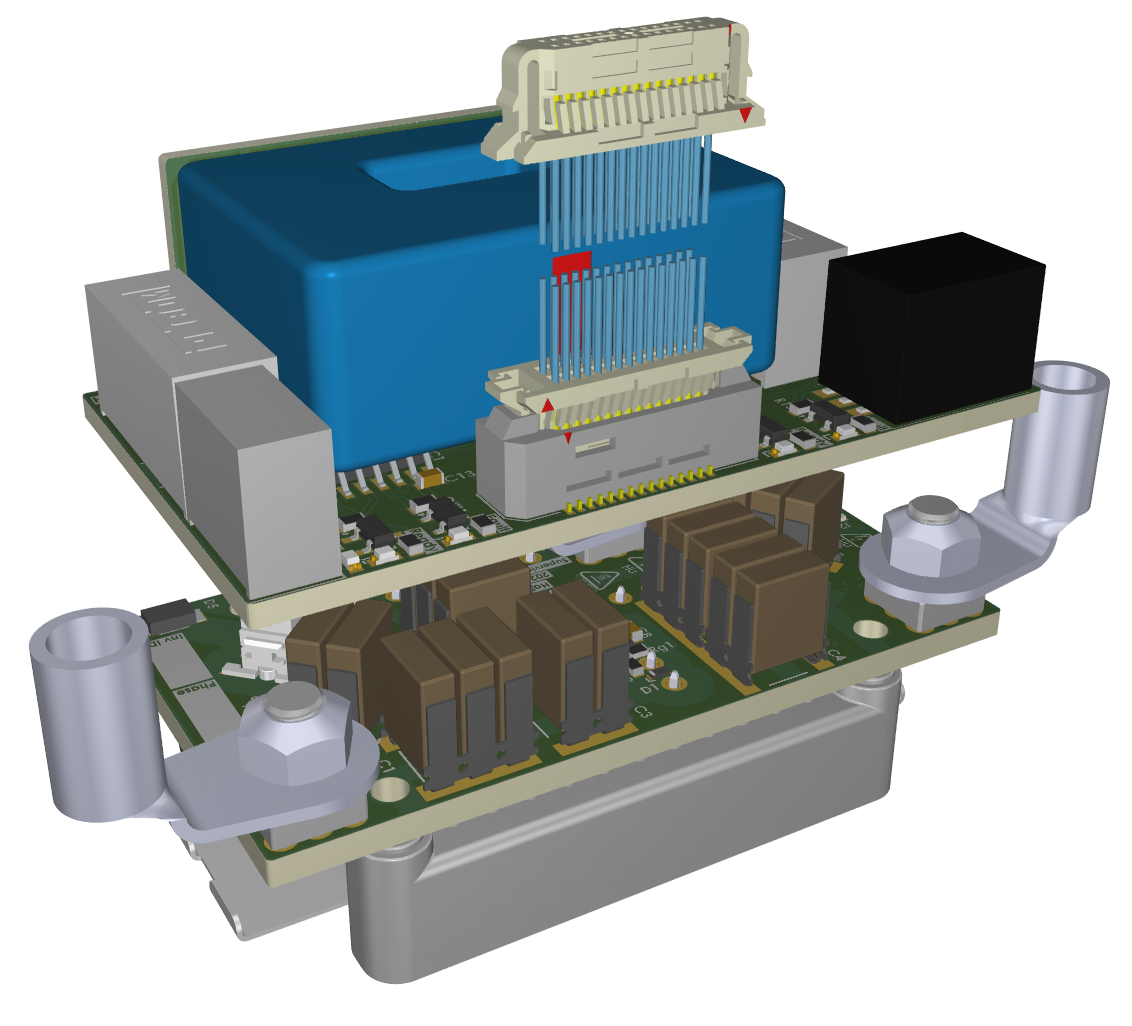
\includegraphics[width=0.8\textwidth]{Figures/Assembly.png}
	\caption{Render of the final leg module.}
	\label{fig:inverter_leg_render}
\end{figure}

\section{Inverter Schematics and Layers}

The resulting schematics and layers of the inverter are presented in the next pages.

\def\excerpt{\subsection{Half Bridge Board Schematic}\label{section:half_bridge_files}}
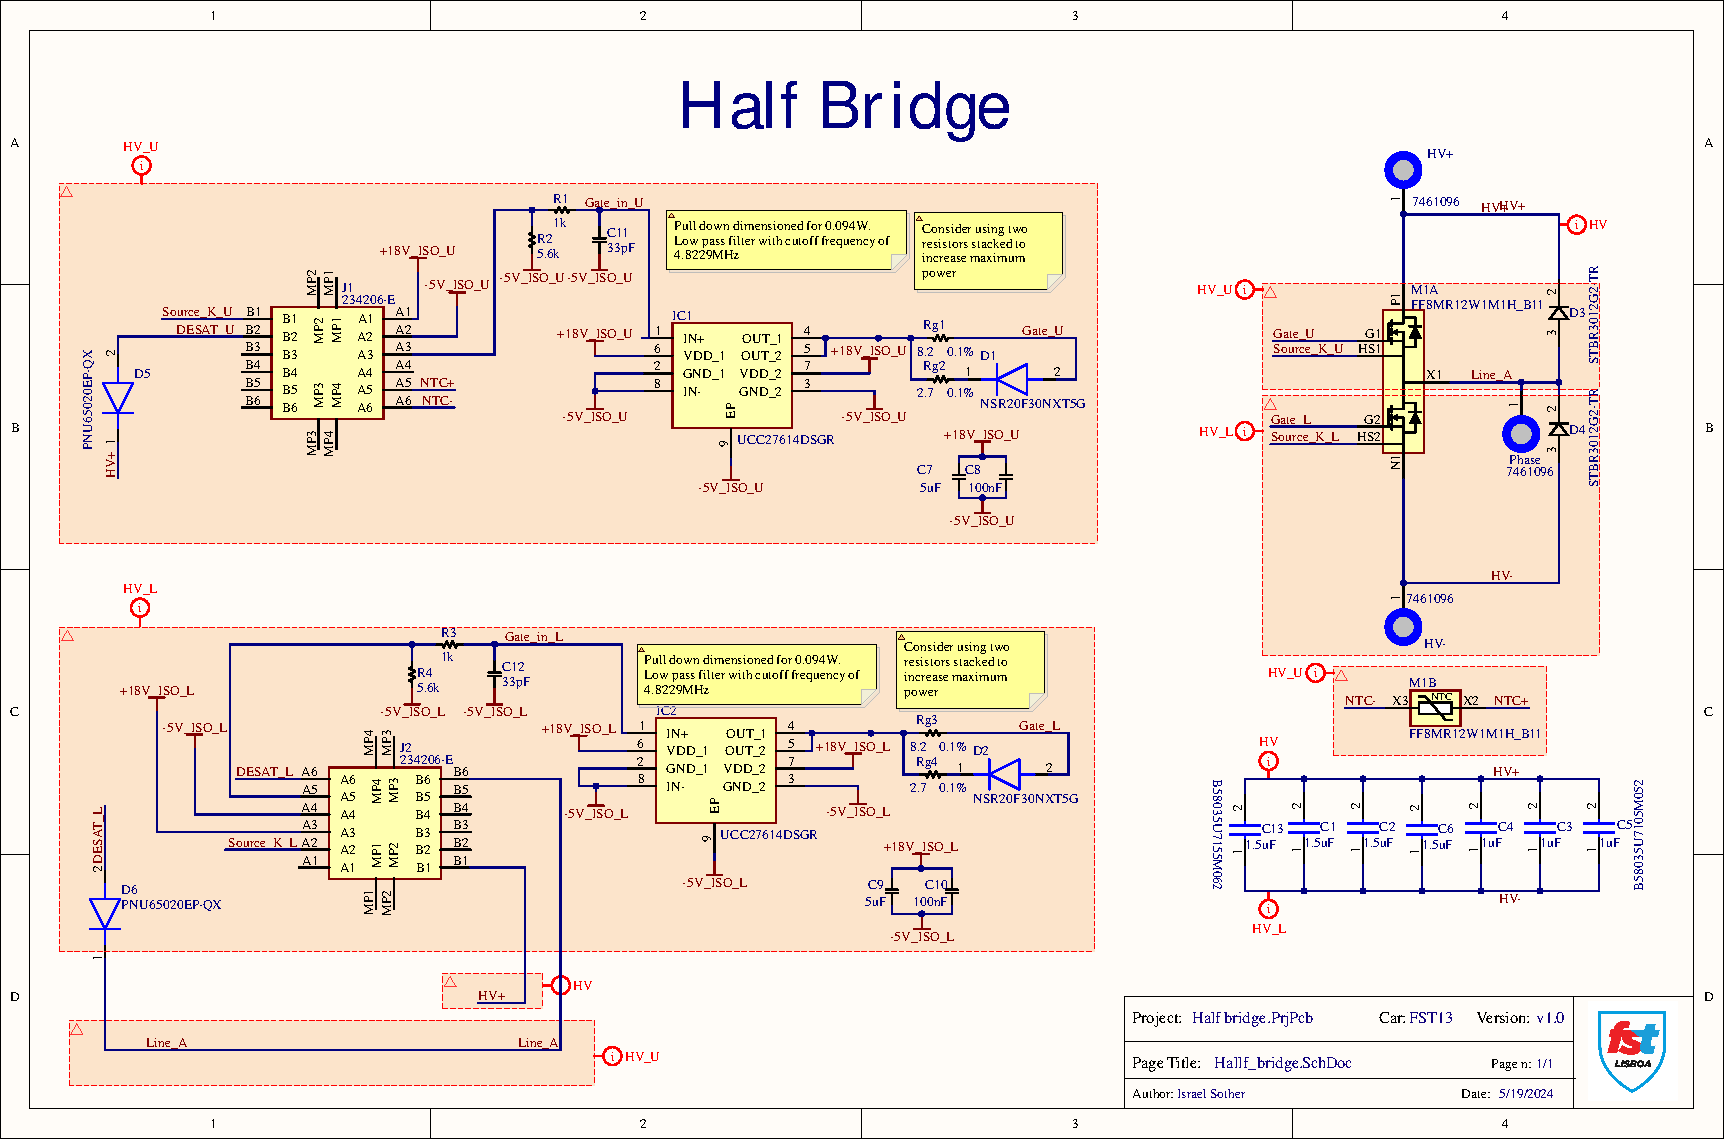
\includepdf[pages={1},nup=1x1,landscape=true,scale=0.8,pagecommand={\excerpt}]{./Appendix/Job3.pdf}
\subsection{Half Bridge Board Layers}
\begin{figure}[H]
	\centering
	\begin{subfigmatrix}{4}
		\subfigure[Top Layer.]{\includegraphics[page=2,width=0.2\textwidth,angle=0,origin=c]{Appendix/Job3.pdf}}
		\subfigure[Inner Layer 1.]{\includegraphics[page=3,width=0.2\textwidth,angle=0,origin=c]{Appendix/Job3.pdf}}
		\subfigure[Inner Layer 2.]{\includegraphics[page=4,width=0.2\textwidth,angle=0,origin=c]{Appendix/Job3.pdf}}
		\subfigure[Inner Layer 3.]{\includegraphics[page=5,width=0.2\textwidth,angle=0,origin=c]{Appendix/Job3.pdf}}
	\end{subfigmatrix}
	\begin{subfigmatrix}{4}
		\subfigure[Inner Layer 4.]{\includegraphics[page=6,width=0.2\textwidth,angle=0,origin=c]{Appendix/Job3.pdf}}
		\subfigure[Inner Layer 5.]{\includegraphics[page=7,width=0.2\textwidth,angle=0,origin=c]{Appendix/Job3.pdf}}
		\subfigure[Inner Layer 6.]{\includegraphics[page=8,width=0.2\textwidth,angle=0,origin=c]{Appendix/Job3.pdf}}
		\subfigure[Bottom Layer.]{\includegraphics[page=9,width=0.2\textwidth,angle=0,origin=c]{Appendix/Job3.pdf}}
	\end{subfigmatrix}
	\caption{Half Bridge Board Layers.}
	\label{fig:half_bridge_board_layers}
\end{figure}

\def\excerpt{\subsection{Gate Driver Board Schematic}\label{section:gate_driver_files}}
\includepdf[pages={1},nup=1x1,landscape=true,scale=0.8,pagecommand={\excerpt}]{./Appendix/Job1.pdf}
\includepdf[pages={2-9},nup=1x1,landscape=true,scale=0.8,pagecommand={}]{./Appendix/Job1.pdf}
\subsection{Gate Driver Board Layers}
\begin{figure}[H]
	\centering
	\begin{subfigmatrix}{2}
		\hfill{ }
		\subfigure[Top Layer.]{\includegraphics[page=10,width=0.35\textwidth,angle=0,origin=c]{./Appendix/Job1.pdf}}
		\subfigure[Inner Layer 1.]{\includegraphics[page=11,width=0.35\textwidth,angle=0,origin=c]{./Appendix/Job1.pdf}}
		\hfill{ }
	\end{subfigmatrix}
	\begin{subfigmatrix}{2}
		\hfill{ }
		\subfigure[Inner Layer 2.]{\includegraphics[page=12,width=0.35\textwidth,angle=0,origin=c]{./Appendix/Job1.pdf}}
		\subfigure[Bottom Layer.]{\includegraphics[page=13,width=0.35\textwidth,angle=0,origin=c]{./Appendix/Job1.pdf}}
		\hfill{ }
	\end{subfigmatrix}
	\caption{Gate Driver Board Layers.}
	\label{fig:gate_driver_board_layers}
\end{figure}

\def\excerpt{\subsection{Current Sensor Board Schematic}\label{section:current_sensor_files}}
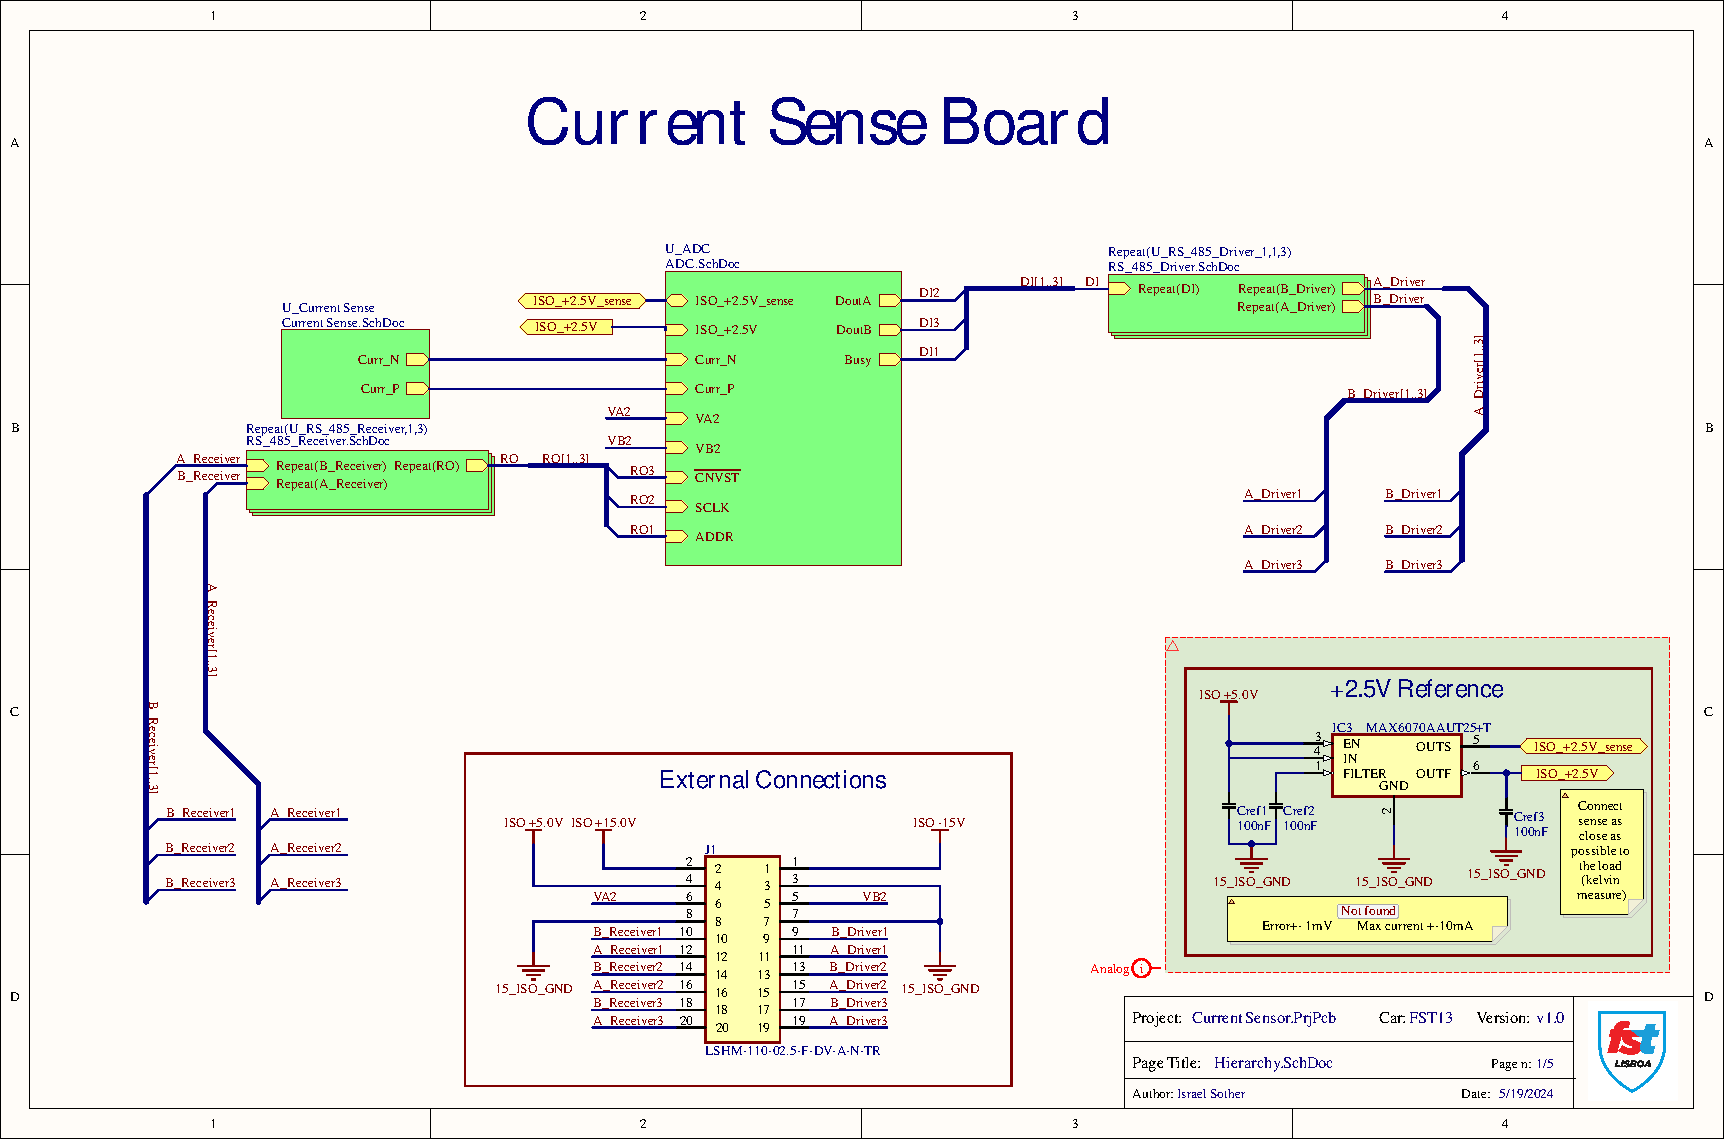
\includepdf[pages={1},nup=1x1,landscape=true,scale=0.8,pagecommand={\excerpt}]{./Appendix/Job2.pdf}
\includepdf[pages={2-5},nup=1x1,landscape=true,scale=0.8,pagecommand={}]{./Appendix/Job2.pdf}
\subsection{Current Sensor Board Layers}
\subsubsection{Top Layer}
\begin{center}
	\includegraphics[page=6,width=0.5\textwidth,angle=90,origin=c]{./Appendix/Job2.pdf}
\end{center}
\subsubsection{Bottom Layer}
\begin{center}
	\includegraphics[page=7,width=0.5\textwidth,angle=90,origin=c]{./Appendix/Job2.pdf}
\end{center}